\documentclass{beamer}

\usepackage[utf8]{inputenc}
% \usepackage{helvet}
% \usepackage[english, ngerman]{babel}
% \usepackage{xltxtra} % XeLaTeX extras
% \usepackage{amsmath}
% \usepackage{fontspec, unicode-math}
% \setsansfont[Mapping=tex-text]{Open Sans Light}
% \setmathfont[version=asana]{Asana Math}

\setbeamertemplate{bibliography item}{\insertbiblabel}

\usecolortheme{tum}
\useoutertheme{tum}

\setbeamerfont{author}{size=\footnotesize}
\setbeamerfont{date}{size=\scriptsize}
\setbeamerfont{date}{size=\scriptsize}

\useinnertheme{rectangles}

\graphicspath{{graphics/}}

\usepackage{pgf}  
\usepackage{tikz}
\logo{\pgfputat{\pgfxy(-0.2, 8.9)}{\pgfbox[right,top]{
\begin{tikzpicture}[y=0.38pt, x=0.38pt,yscale=-1, inner sep=0pt, outer sep=0pt]
\begin{scope}[cm={{1.25,0.0,0.0,-1.25,(0.0,35.4325)}}]
    \path[fill=tum,nonzero rule] (4.8090,23.2950) -- (4.8090,-0.0020) --
      (9.8590,-0.0020) -- (9.8590,23.2600) -- (15.4730,23.2600) -- (15.4730,-0.0020)
      -- (31.5390,-0.0020) -- (31.5390,23.0140) -- (37.2580,23.0140) --
      (37.2580,0.0060) -- (42.5550,0.0060) -- (42.5550,23.0140) -- (48.3440,23.0140)
      -- (48.3440,0.0060) -- (53.6410,0.0060) -- (53.6410,28.3460) --
      (26.4530,28.3460) -- (26.4530,5.1580) -- (20.6290,5.1580) -- (20.6290,28.3110)
      -- (-0.0000,28.3110) -- (-0.0000,23.2950) -- (4.8090,23.2950) -- cycle;
\end{scope}
\end{tikzpicture}
}}}
\setbeamertemplate{footline}[frame number]
\setbeamertemplate{navigation symbols}{}%remove navigation symbols
\setbeamertemplate{title page}
{
	\vbox{}
	\vfill
	\begin{flushleft}
		\begin{beamercolorbox}[sep=8pt,left]{title}
			\usebeamerfont{title}\inserttitle\par%
			\ifx\insertsubtitle\@empty%
			\else%
				\vskip0.25em%
				{\usebeamerfont{subtitle}\usebeamercolor[fg]{subtitle}\insertsubtitle\par}%
			\fi%
    	\end{beamercolorbox}%
    	\vskip1em\par
		\begin{beamercolorbox}[sep=8pt,left]{author}
		\usebeamerfont{author}\insertauthor
		\end{beamercolorbox}
		\begin{beamercolorbox}[sep=8pt,left]{institute}
		\usebeamerfont{institute}\insertinstitute
		\end{beamercolorbox}
		\begin{beamercolorbox}[sep=8pt,left]{date}
		\usebeamerfont{date}\insertdate
		\end{beamercolorbox}\vskip0.5em
		{\usebeamercolor[fg]{titlegraphic}\inserttitlegraphic\par}
	\end{flushleft}
	\vfill
}

\mode<presentation>

\title{LBM for Rarefied Gas Flows}
\subtitle{Seminar: Lattice Boltzmann Methods}

\author{Gerasimos Chourdakis}
\institute[TUM Informatics]{Fakult\"at f\"ur Informatik - Technische Universit\"at M\"unchen}

\date{June 18, 2015}

\begin{document}

\begin{frame}
  \titlepage
\end{frame}

\begin{frame}
  \frametitle{Agenda}
  \tableofcontents
\end{frame}


\section{Introduction}

\begin{frame}
  \frametitle{Motivation}

  \begin{itemize}
   \item The Navier-Stokes equations assume continuity.
   \item The no-slip boundary conditions do not always apply. 
   \item Micro(nano)-electro-mechanical systems (MEMS): far from continuity, slip-velocity observed.
  \end{itemize}
\end{frame}

\begin{frame}
  \frametitle{Is everything continuous?}
  
  The matter consists of small discrete particles,
  though it seems to be continuous.

  \begin{itemize}
   \item How to quantify the ``continuity''?
   \item What are the limits of this assumption?
   \item Can we always apply the Navier-Stokes equations?
   \item Can we always apply a lattice Boltzmann menthod?
   \item If not, what can we do about this?
  \end{itemize}
\end{frame}

\begin{frame}
 \frametitle{Example: micropumps}
 \begin{figure}
  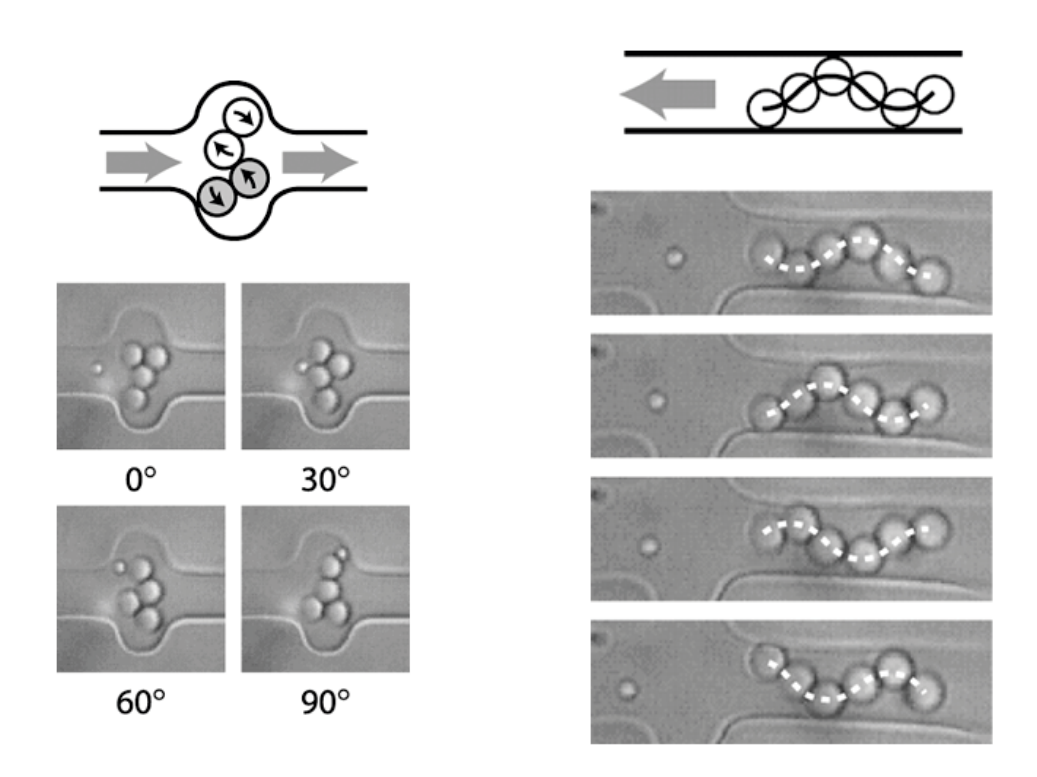
\includegraphics[scale=0.2]{microfluids_pumps}
  \caption{Colloidal micropumps.\,\footnotemark}
 \end{figure}
\footnotetext{Karniadakis et al. - 2005~\cite{Karniadakis_Microflows}}
\end{frame}

\section{Flow regimes}

\begin{frame}
 \frametitle{Mean Free Path}
 
 Mean Free Path: the average distance that the molecules 
 of a gas are travelling without taking part in collisions.
 
 For hard-sphere gases in thermodynamic equilibrium:
  \begin{equation}
    \lambda = \frac{1}{\sqrt{2} \pi \cdot n_\mathrm{g} \cdot d^2}
    \label{eq:MFP}
  \end{equation}
  $d$: mean molecular diameter, $n_\mathrm{g}$: number density
  
  
  Example (atmospheric conditions):
  
  $\lambda_{\mathrm{air}} = 6.111\cdot10^{-8}\,\mathrm{m}$
  
  $\lambda_{\mathrm{He}} = 17.651\cdot10^{-8}\,\mathrm{m}$
 
\end{frame}


\begin{frame}
 \frametitle{The Knudsen number}
 
 Knudsen number = Mean Free Path / characteristic length
 
 \begin{equation}
 \mathrm{Kn} := \frac{\lambda}{L_0}
 \label{eq:Kn_def}
\end{equation}
 
 The characteristic length can be, e.g.\@, the width of a channel.

\end{frame}


\begin{frame}
 \frametitle{Flow regimes}
 
 Empirical Knudsen number ranges:
 \begin{description}[Free molecular]
  \item[Continuous] $\mathrm{Kn}<10^{-2}$ (or $\mathrm{Kn}<10^{-3}$)
  \item[Slip] $10^{-2} < \mathrm{Kn} < 10^{-1} $ (thermodynamic equilibrium breaks)
  \item[Transition] $10^{-1} < \mathrm{Kn} < 10 $ (continuity assumption breaks)
  \item[Free molecular] $10 < \mathrm{Kn}$ (almost no intermolecular collisions)
 \end{description}

 Also, mixed flow regimes for scenarios with very different scales.
\end{frame}

\begin{frame}
 \frametitle{Flow regimes (2)}
 
 \begin{figure}
  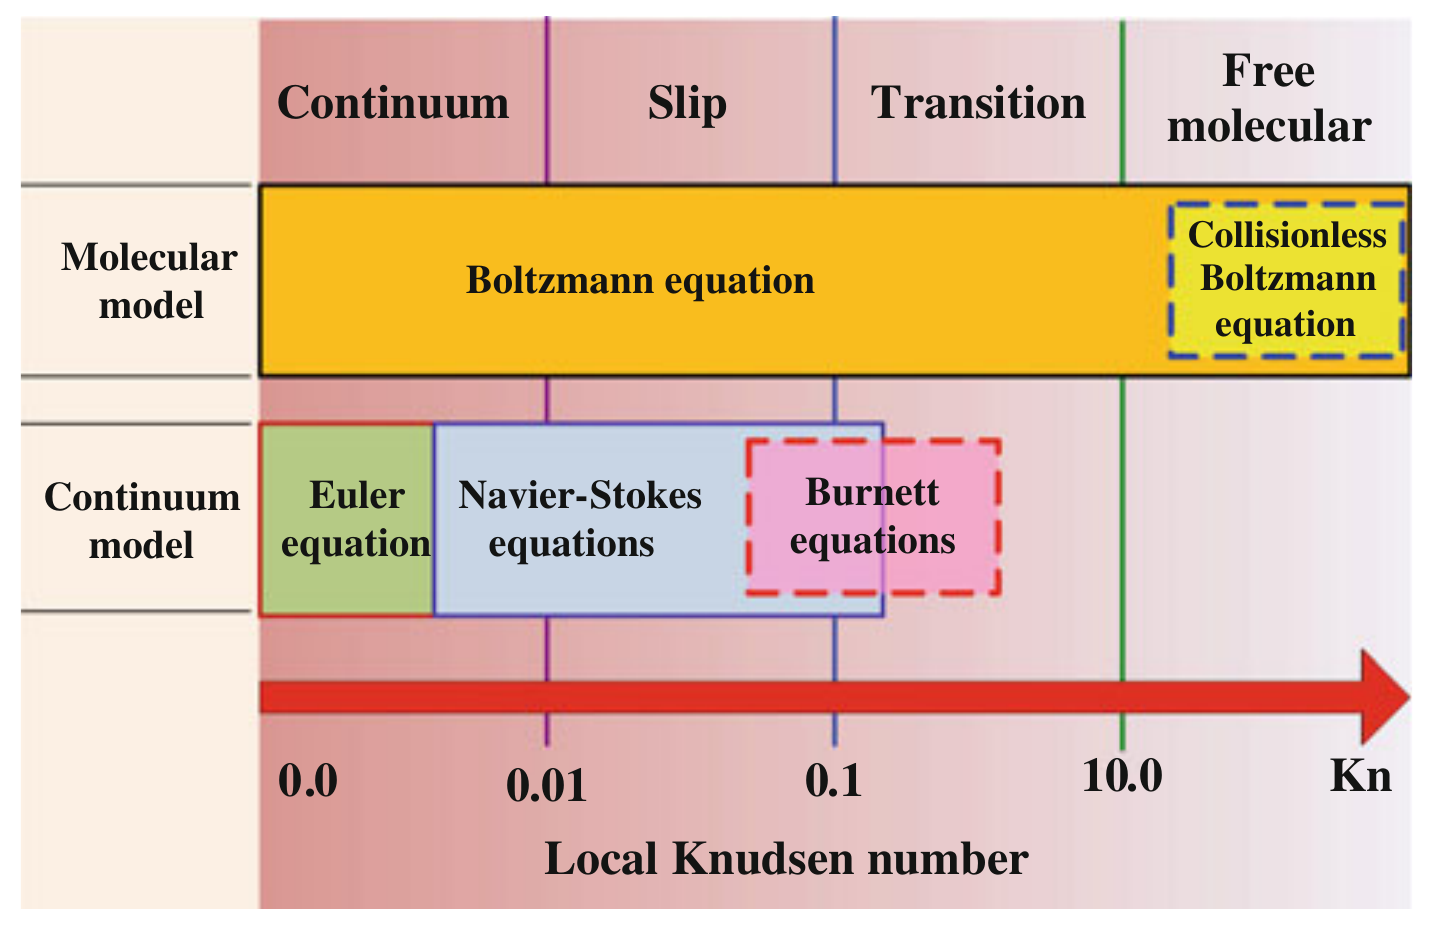
\includegraphics[scale=0.15]{flow_regimes}
  \caption{Gas flow regimes and limits of different CFD approaches.\,\footnotemark}
 \end{figure}
  \footnotetext{Zhang et al. - 2012~\cite{Zhang2012}}
 
\end{frame}


\section{Extending LBM to the slip regime}

\begin{frame}
 \frametitle{Extending LBM to the slip regime}
 The ``classical'' Bhatnagar-Gross-Krook LBM with bounce-back boundary conditions
 has some problems:
 \begin{itemize}
  \item The boundary conditions depend on the viscosity
  \item The observed ``slip velocity'' is a numerical artifact, 
  it is constant at the wall, without depending on the Knudsen number\,\footnote{Verhaeghe - 2009~\cite{Verhaeghe2009}}
 \end{itemize}

 Solutions:
 \begin{itemize}
  \item Multiple-Relaxation-Time collision
  \item Slip-velocity models
  \item Virtual wall collisions and other ideas
 \end{itemize}
\end{frame}

\begin{frame}
 \frametitle{Multiple-Relaxation-Time}
 General form of the LB equation:
 \begin{equation}
 \mathbf{f}(\mathbf{r}_j + \mathbf{c}\delta_\mathrm{t}, t+\delta_\mathrm{t}) = \mathbf{f}(\mathbf{r}_j, t) + \mathbf{\Omega}[\mathbf{f}(\mathbf{r}_j, t)] + \mathbf{F}(\mathbf{r}_j, t)
\end{equation}

MRT collision operator:
\begin{equation}
 \mathbf{\Omega} = - \mathrm{M}^{-1} \cdot \mathrm{S} \cdot [\mathbf{m} - \mathbf{m}^\mathrm{(eq)}] 
 \textrm{ , \ }
 \mathbf{m} = \mathrm{M} \cdot \mathbf{f}
\end{equation}
where $\mathbf{m}$ is the moment space (and $\mathbf{m}^\mathrm{(eq)}$ the respective equilibria), $\mathrm{S}$ a positive-definite matrix of
the relaxation rates and $\mathrm{M}$ the matrix that transforms $\mathbf{f}$ to
their moments
\end{frame}

\begin{frame}
 \frametitle{Slip-velocity models}
 How does the velocity change near the wall?
 
 A first-order model for the slip regime:
 \begin{equation}
 u|_\mathrm{wall} = \sigma \mathrm{Kn} L_0 \frac{\partial u_\mathrm{wall}}{\partial y} \textrm{, \ } \sigma := (2 - \sigma_\nu)/\sigma_\nu 
 \label{eq:slip_1order}
\end{equation}
 $\sigma_\nu \in (0,1]$: tangential momentum accommodation coefficient~\cite{Verhaeghe2009}.
 
 \begin{figure}
  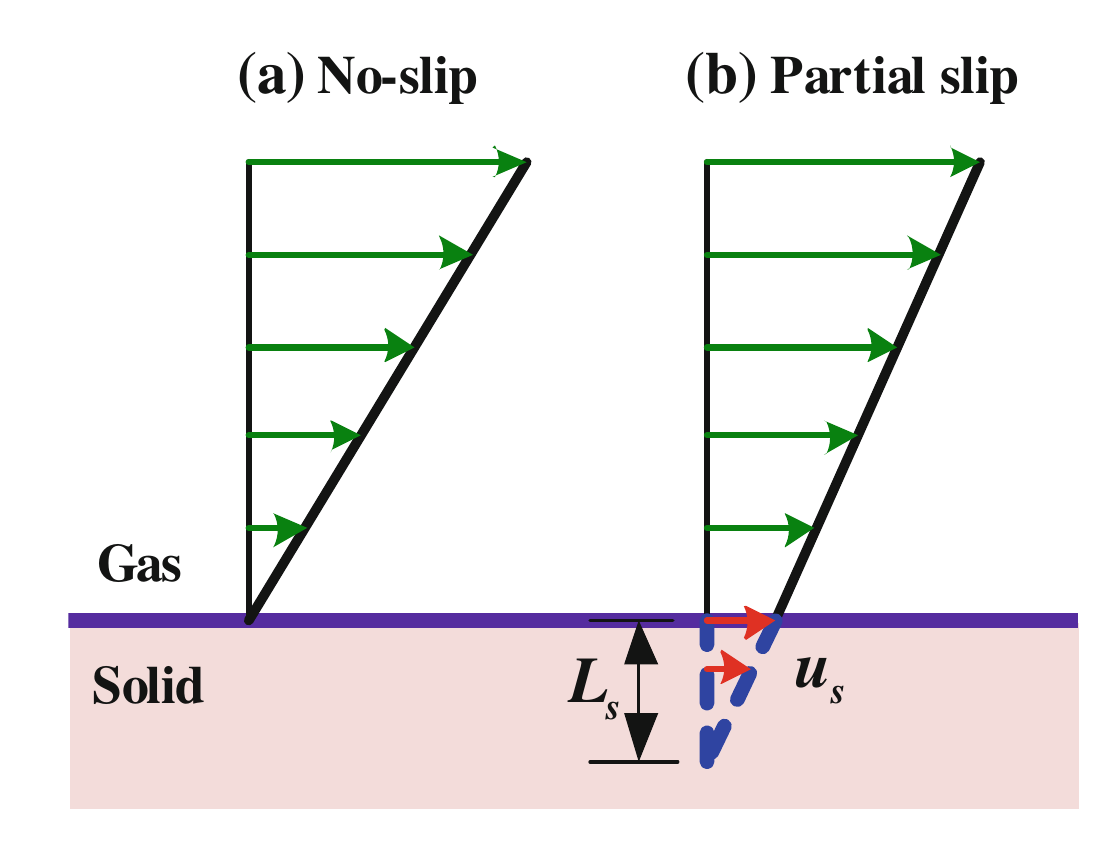
\includegraphics[scale=0.1]{Zhang-slip}
  \caption{A linear slip-velocity model~\footnote{Zhang et al. - 2012~\cite{Zhang2012}}}
 \end{figure}

\end{frame}

\begin{frame}
 \frametitle{Boundary conditions}
 Analytic solution of the lattice Boltzmann equation for the incompressible Poiseuille flow (dimensionless):
 \begin{equation}
 \tilde{u}(\tilde{y}) = 4\tilde{y}(1-\tilde{y}) { \color{tum} \ + \  \tilde{U}_\mathrm{slip} }
\end{equation}
where: \\ 
$\tilde{u} := (u + G\delta_\mathrm{t} / 2) / U_\mathrm{max}$, \\
$G := |\nabla p / \rho|$ (acceleration due to a constant pressure gradient), \\
$\tilde{U}_\mathrm{slip} := U_\mathrm{slip} / U_\mathrm{max}$, \\
$\tilde{y} := (j-1/2)/N_\mathrm{y}$.
\end{frame}


\begin{frame}
 \frametitle{Bounce-Back boundary conditions}
 For smooth surfaces, the momentum is reversed:
 \begin{equation}
  f_i(t_{n+1}) = f_{inv(i)}^*(t_n)
 \end{equation}
 
 \begin{equation}
  U_\mathrm{slip}^\mathrm{B} = \frac{1}{4} \Big(\frac{8}{\tau_q} - \frac{8-\tau_s}{2-\tau_s} \Big) G \delta_\mathrm{t}
 \end{equation}
 
 $\tau_s$, $\tau_q$: relaxation rates for the stresses and the energy fluxes.
 
 No-slip ($U_\mathrm{slip}^\mathrm{B} = 0$) if:
 \begin{equation}
 \tau_q = \frac{8(2-\tau_s)}{(8-\tau_s)}
 \end{equation}
\end{frame}

\begin{frame}
 \frametitle{Diffusive boundary conditions}
 For non-smooth surfaces, the molecules are reflected to random directions:
 \begin{equation}
 f_i = \frac{\sum_{\mathbf{c}_k} | \mathbf{c}_k \cdot \hat{\mathbf{n}}| f_k^* }
 { \sum_{\mathbf{c}_k} | \mathbf{c}_k \cdot \hat{\mathbf{n}} | f_k^\mathrm{(eq)}(\rho_\mathrm{wall}, \mathbf{u}_\mathrm{wall})  }
 f_{inv(i)}^{\mathrm{(eq)}}(\rho_\mathrm{wall}, \mathbf{u}_\mathrm{wall}) := f_i^\mathrm{D} \textrm{, \ } \mathbf{c}_k \cdot \hat{\mathbf{n}} < 0
\end{equation}
$\hat{\mathbf{n}}$: the normal to the wall unit vector, \\
$\mathbf{c}_k$: incidental velocities defined by $ \mathbf{c}_k \cdot \hat{\mathbf{n}} < 0$ and $\rho_\mathrm{wall}$,\\
$\mathbf{u}_\mathrm{wall}$: density and velocity at the wall

\begin{equation}
 U_\mathrm{slip}^\mathrm{D} = U_\mathrm{slip}^\mathrm{B} + \frac{3}{2}N_\mathrm{y} G \delta_\mathrm{t} = U_\mathrm{slip}^\mathrm{B} + \frac{3}{2} \frac{L_0 G}{c} \textrm{, \ } c:=\delta_\mathrm{x} / \delta_\mathrm{t}
\end{equation}
\end{frame}

\begin{frame}
 \frametitle{Diffusive bounce-back boundary conditions}
 
 Combining the BB and the Diffusive boundary conditions:
 \begin{equation}
 f_i(t_{n+1}) = \beta f_{inv(i)}^{*} (t_n) + (1-\beta)f_i^\mathrm{D}(t_n) \textrm{, \ } \beta \in [0,1]
\end{equation}

\begin{equation}
 U_\mathrm{slip}^\mathrm{BD} = U_\mathrm{slip}^\mathrm{B} + \frac{3}{2} \frac{(1-\beta)}{(1+\beta)} N_\mathrm{y} G \delta_\mathrm{t}
 = U_\mathrm{slip}^\mathrm{B} + \frac{3}{2} \frac{(1-\beta)}{(1+\beta)} \frac{L_0 G}{c}
\end{equation}

Verhaeghe et al.~\cite{Verhaeghe2009}:
\begin{equation}
 \beta = \frac{3\mu - \mathrm{Kn} L_0 c \bar{\rho}_\mathrm{out} }{3\mu + \mathrm{Kn} L_0 c \bar{\rho}_\mathrm{out} }
 \label{eq:betaBD}
\end{equation}
\end{frame}

\begin{frame}
 \frametitle{Specular reflective bounce-back boundary conditions}
 Combining the Specular reflective (``free-slip'') and the bounce-back boundary conditions:
\begin{equation}
 U_\mathrm{slip}^\mathrm{BR} = U_\mathrm{slip}^\mathrm{B} + \frac{3}{2} \frac{(1-\beta)}{\beta} N_\mathrm{y} G \delta_\mathrm{t}
 = U_\mathrm{slip}^\mathrm{B} + \frac{3}{2} \frac{(1-\beta)}{\beta} \frac{L_0 G}{c}
\end{equation}
\end{frame}

\begin{frame}
 \frametitle{Some results (slip regime)}
 \begin{figure}
  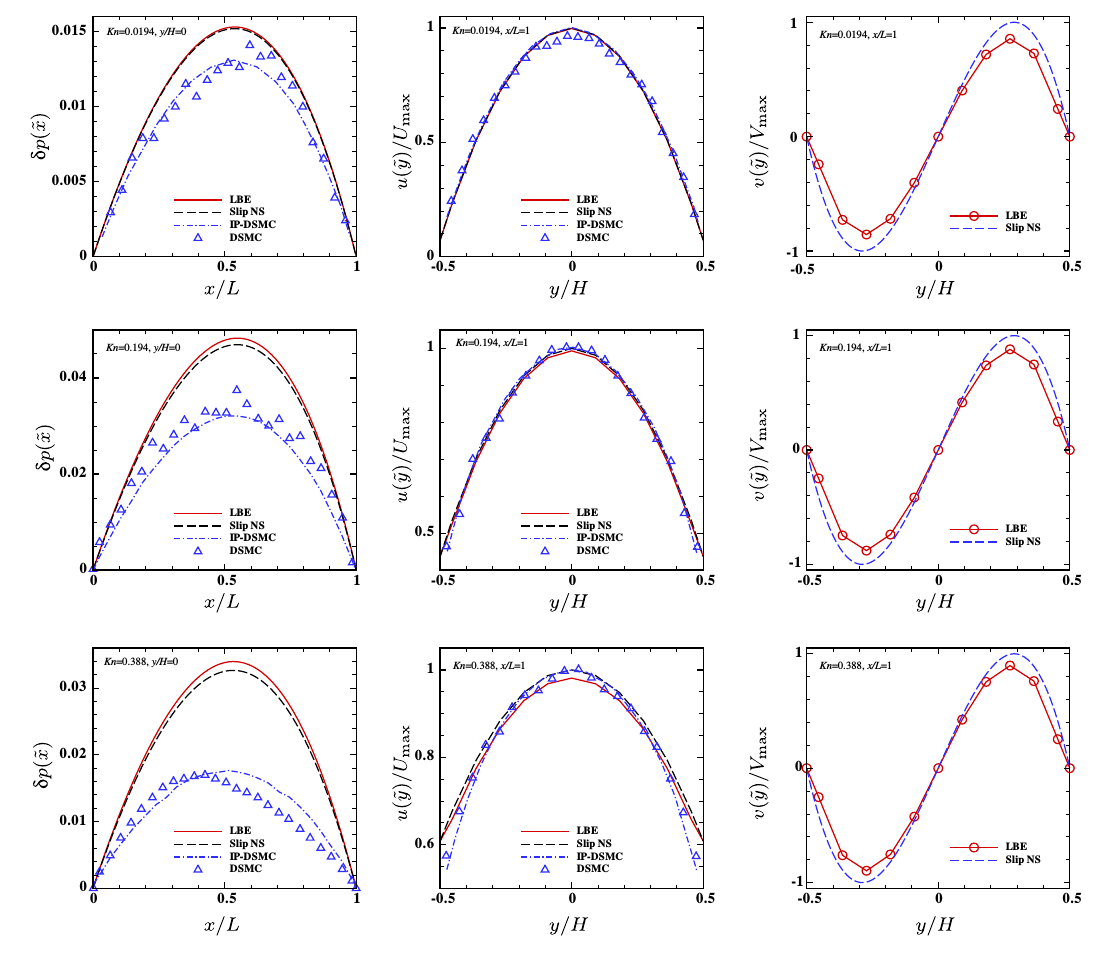
\includegraphics[scale=0.2]{Verhaeghe}
  \caption{Results of Verhaeghe et al.~\cite{Verhaeghe2009} for the slip regime, compared to the slip Navier-Stokes, IP-DSMC and DSMC.}
 \end{figure}
\end{frame}

\section{LBM in the transition regime}

\begin{frame}
 \frametitle{LBM in the transition regime (1)}
 
 Near the walls, the MFP is shorter and the viscosity decreases:
 \begin{equation}
 \mu_\mathrm{e} = \mu_0 \frac{1}{1 + \alpha \mathrm{Kn}} \textrm{, \ } \alpha \approx 2
\end{equation}
 
 Effective MFP:
 \begin{equation}
 \lambda_\mathrm{e} = \frac{\mu_\mathrm{e}}{p} \cdot \sqrt{\frac{\pi R T}{2}}
 \end{equation}
 
 Second-order slip-velocity model\footnote{Li et al. - 2011~\cite{Li2011}, Zhang et al. - 2012~\cite{Zhang2012}}:
 \begin{equation}
 U_\mathrm{slip} = B_1 \sigma_\nu \lambda_\mathrm{e} \frac{\partial u}{\partial y} \Big|_\mathrm{wall} - B_2 \lambda_\mathrm{e}^2 \frac{\partial^2 u}{\partial y^2} \Big|_\mathrm{wall} \textrm{ , \ } \sigma_\nu = (2 - \sigma)/\sigma
  \label{eq:slip2}
 \end{equation} 
\end{frame}

\begin{frame}
 \frametitle{LBM in the transition regime (2)}
 Li et al.~\cite{Li2011} use MRT and set:
 \begin{equation}
 \tau_s = \frac{1}{2} + \sqrt{\frac{6}{\pi}} \frac{N \mathrm{Kn}}{(1+\alpha \mathrm{Kn})} \textrm{ , \ } N=H/\delta_\mathrm{x}
\end{equation}
\begin{equation}
 \tau_q = \frac{1}{2} + \frac{3 + 4 \pi \tilde{\tau}_s^2 B_2}{16 \tilde{\tau}_s } \textrm{ , \ } \tilde{\tau}_s = \tau_s - 0.5
\end{equation}

For the diffusive bounce-back boundary conditions:
\begin{equation}
 \beta = \frac{1}{1 + B_1 \sigma_\nu \sqrt{\pi / 6}}
\end{equation}
\end{frame}

\begin{frame}
 \frametitle{Some results (transition regime)}
 \begin{figure}
  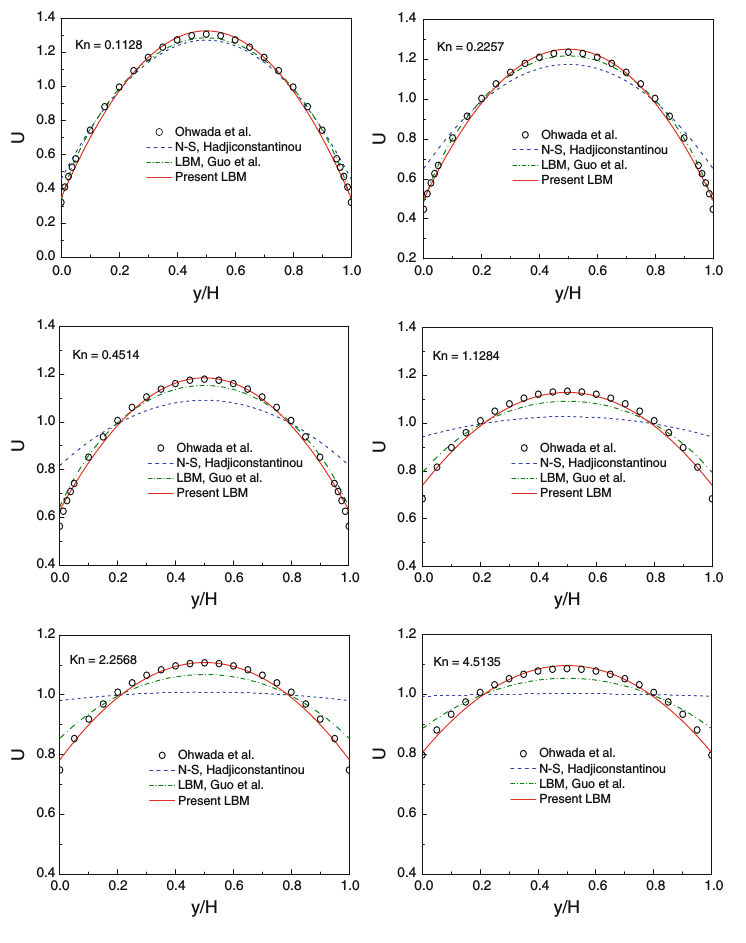
\includegraphics[scale=0.2]{Li}
  \caption{Results of Li et al.~\cite{Li2011} for the transition regime, compared to the Navier-Stokes and other approaches.}
 \end{figure}
\end{frame}

\section{A stochastic model for finite Knudsen numbers}

\begin{frame}
 \frametitle{Virtual wall collisions (Toschi and Succi) (1)}
 \begin{figure}
  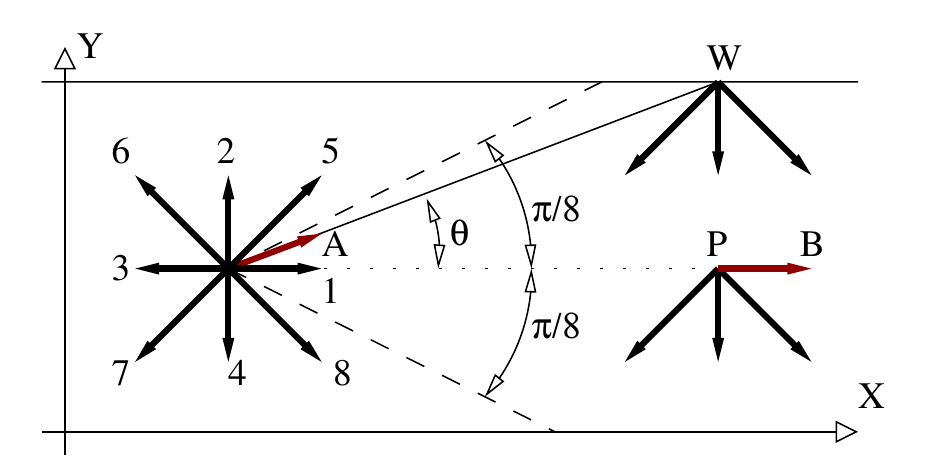
\includegraphics[scale=0.3]{Toschi}
  \caption{All the molecules that were going to travel within the %
 		$-\pi/8 < \theta < \pi/8$ range are actually mapped to %
 		a single direction. Because this direction is parallel to the flow, %
 		and because the intermolecular collisions are rare, these molecules %
 		will never collide with the walls and they will continue accelerating.}
 \end{figure}

\end{frame}

\begin{frame}
 \frametitle{Virtual wall collisions (Toschi and Succi) (2)}
 Probability of virtual wall collision: \\
 probability to { \color{tum} avoid intermolecular collisions } before hitting
the wall, multiplied by the probability to { \color{red} collide with the wall in a time step }:
\begin{equation}
 p(x, y; t) = { \color{tum} \exp( -1/\mathrm{Kn} ) } \cdot { \color{red} \Big( 1 - \exp \Big( - \frac{c \cdot \mathrm{d}t \cdot \sin(\theta(x,y))}{H} \Big)   \Big) }
\end{equation}

After colliding with the upper boundary:
\begin{eqnarray*}
 f'_1 = f_1(1 {\color{red}-}p) &\textrm{, \ \ } f'_{7,8} = f_{7,8} {\color{green}+} p f_1 / 6 &\textrm{, \ \ } f'_4 = f_4 {\color{green}+} 4 p f_1 / 6 \\
 f'_3 = f_3(1{\color{red}-}p) &\textrm{, \ \ } f'_{5,6} = f_{5,6} {\color{green}+} p f_3 / 6 &\textrm{, \ \ } f'_2 = f_2 {\color{green}+} 4 p f_3 / 6
\end{eqnarray*}
In this way, particles are re-distributed to other directions.
\end{frame}

\begin{frame}
 \frametitle{Some results (Virtual wall collisions)}
 \begin{figure}
  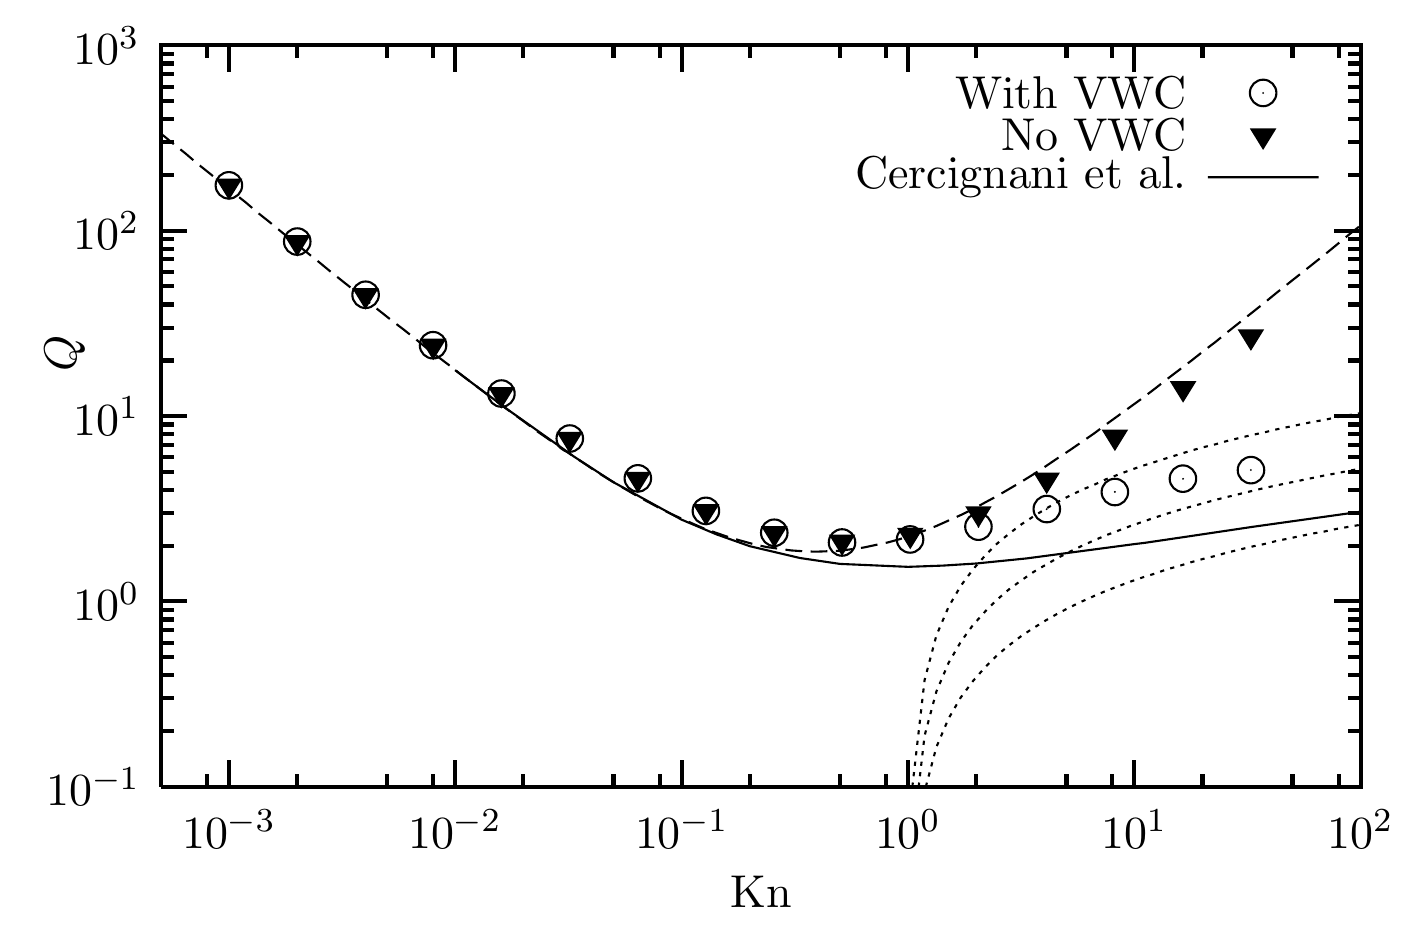
\includegraphics[scale=0.2]{Toschi-AK}
  \caption{Results of Toschi and Succi~\cite{Toschi2005} (mass flux) with Ansumali-Karlin BC, with and without virtual-wall-collisions, compared to a prediction.}
 \end{figure}
\end{frame}


\section{Conclusion}

\begin{frame}
 \frametitle{Conclusions}
 \begin{itemize}
  \item The continuous methods are not the correct tool for microfluids!
  \item LBM can be applied, MRT collision is suggested.
  \item LBM can work well in the slip and the transition regime, by adjusting the boundary conditions.
  \item Virtual wall collisions can fix the freely-accelerating beams.
  \item What happens in the free-molecular regime?
 \end{itemize}

\end{frame}

\nocite{Barber2006, Michalis2010}

\begin{frame}[allowframebreaks]
 \frametitle{References}
 \bibliographystyle{plain}
 \bibliography{../references}
\end{frame}

\end{document}